%setting document class
\documentclass[a4paper,10pt]{article}

%importing packages
\usepackage[utf8]{inputenc}
\usepackage[T1]{fontenc,url}
\usepackage[english]{babel}
\usepackage{gensymb}
\usepackage{amsmath}
\usepackage{amssymb}
\usepackage{commath}
\usepackage{physics}
\usepackage{float}
\usepackage{listings}
\usepackage{graphicx}
\usepackage{titlesec}
\usepackage{datetime}

%formatting
\newdateformat{mydate}{\THEDAY. \monthname,  \THEYEAR}

\titleformat*{\section}{\centering \textsc}
\titlelabel{\thetitle.\quad}

\titleformat{\subsection}[runin]{\normalfont\bfseries}{\thesubsection}{1em}{}
\titleformat{\subsubsection}[runin]{\normalfont\normalsize\bfseries}{\thesubsubsection}{1em}{}


%front page title/author setup
 \title{AST 4320 - Assignment 2
}
 \date{\normalsize{\textsc{\mydate\today}} }
 \author{\textsc{\small{Metin San}}}



%starting the document
\begin{document}
\maketitle

\bigskip

\section*{Exercise 1.}

We will now consider the top-hat smoothing function in 1D, also known as the window function $W(x)$. The top-hat smoothing function is expressed as

\begin{equation}\label{eq:1}
    W(x) = 
    \begin{cases}
    1, & \text{if } \abs{x} < R\\
    0, & \text{otherwise}
    \end{cases},
\end{equation}

\noindent where $R$ is the smoothing scale. We are interested in computing the Fourier conjugate $\Tilde{W}$ of the smoothing function. The Fourier transformation of a function $f(x)$ is given as

\begin{equation}\label{eq:2}
    \Tilde{f}(k) = \int_{-\infty}^{\infty} f(x) e^{-ikx} dx.
\end{equation}

\noindent Applying this transformation to $W(x)$ gives us the following expression to solve

\[
    \Tilde{W}(k) = \int_{-\infty}^{\infty} W(x) e^{-ikx} dx.
\]

\noindent If we insert for the definition of $W(x)$, we see that only the non-zero contributions occur in the limits $R$ to $-R$. This reduces our expression to

\[
    \Tilde{W}(k) = \int_{-R}^{R} e^{-ikx} dx.
\]

\noindent This is a trivial integral to compute. Doing so results in

\[
    \Tilde{W}(k) = -\frac{1}{ik} \left[ e^{-ikx} \right]_{-R}^R = \frac{1}{ik} \left[ e^{ikR} - e^{-ikR} \right].
\]

\noindent From Euler's formula, we know that 

\[
    \sin(kx) = \frac{e^{ikx} - e^{-ikx}}{2i}.
\]

\noindent We see that this can be substituted into the bracket on the right hand side, which leaves us with the final expression

\begin{equation}\label{eq:3}
    \Tilde{W}(k) = \frac{2}{k} \sin(kR).
\end{equation}

\noindent We can now study this quantity. We start by plotting equation \eqref{eq:3} for wavenumbers $k \in [-4\pi , 4\pi]$. The results are seen in figure \ref{fig:1}. We are also interested in knowing what the full width at half the maximum is (FWHM). This quantity is given as FWHM = $2 \sqrt{2\ln 2} \sigma$, where $\sigma$ is the standard deviation in the distribution. However, since we have a non-gaussian distribution with multiple amplitudes, we will have to find the value numerically. We do so by writing a short script in python which finds the the value of $k$ at half the maximum.

We find that the FWHM of the Fourier conjugate of $W(x)$ with smoothing scale $R = 2$ is FWHM $= 1.899$.


\begin{figure}[h]
    \centering
    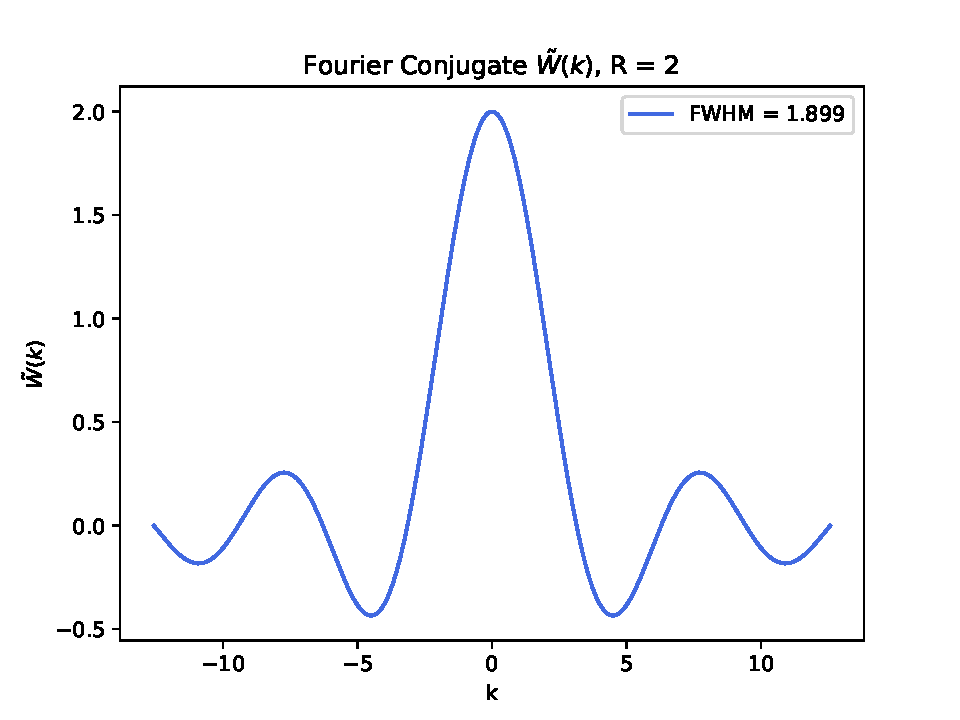
\includegraphics[width=0.8\linewidth]{Figures/Window.pdf}
    \caption{Top-hat smoothing function in 1D with a smoothing scale $R = 2$.}
    \label{fig:1}
\end{figure}

\section*{Exercise 2.}

We will now look into the random walk process. We will consider a power spectrum on the form $P(k) = k$ and extract random numbers from Gaussian random distributions. We define the variance as a function of scale as

\begin{equation}\label{eq:4}
\sigma^2 (S_c) = \frac{\pi}{S_c^4},
\end{equation}

\noindent where $S_c$, the smoothing scale is given as 

\begin{equation}\label{eq:5}
    S_c = \frac{2\pi}{k}.
\end{equation}

The initial condition of $k$ is found by requiring that we start at a radius so that $\sigma^2 (S_c) = \sigma^2 (S_1) < 10^{-4}$. We can find an expression for $k$ which only depends on $\sigma$ by solving equations for $k$. Doing so leaves us with

\begin{equation}
    k = 2\pi \left( \frac{\pi}{\sigma^2} \right)^{-1/4}.
\end{equation}

\noindent This can then be inserted back into equation \eqref{eq:5}, which leaves us with our initial scale

\begin{equation}
    S_1 = \left( \frac{\pi}{\sigma^2} \right)^{1/4}.
\end{equation}

\noindent By then inserting for a initial sigma $\sigma < 10^{-4}$, for instance $0.9 \cross 10^{-4}$, we get our initial $S_1 = 13.66$.

We start by creating an algorithm which first calculates the variance, $\sigma^2$ in equation \eqref{eq:4} using the initial scale $S_1$. It then subtracts a small value $\epsilon$ from the scale $S_c$. It proceeds by computing a new variance using the new $S_c$ value. It then finds the difference in variance between these two variances $\sigma^2_{12} = \sigma^2(S_2) - \sigma^2(s_1)$. It then uses numpy's \textit{random.normal} function which extracts a random normal distributed number $\delta$ with the above variance $\sigma^2_{12}$. This is then continued until the scale $S_c$ drops to $S_c = 1$ at which point we extract the final $\delta$ value corresponding to $S_c = 1$. 

This whole sequence is computed $10^5$ times. The distribution of the extracted $\delta$ are then plotted in a histogram  which is seen in figure \ref{fig:2}.
\begin{figure}[h]
    \centering
    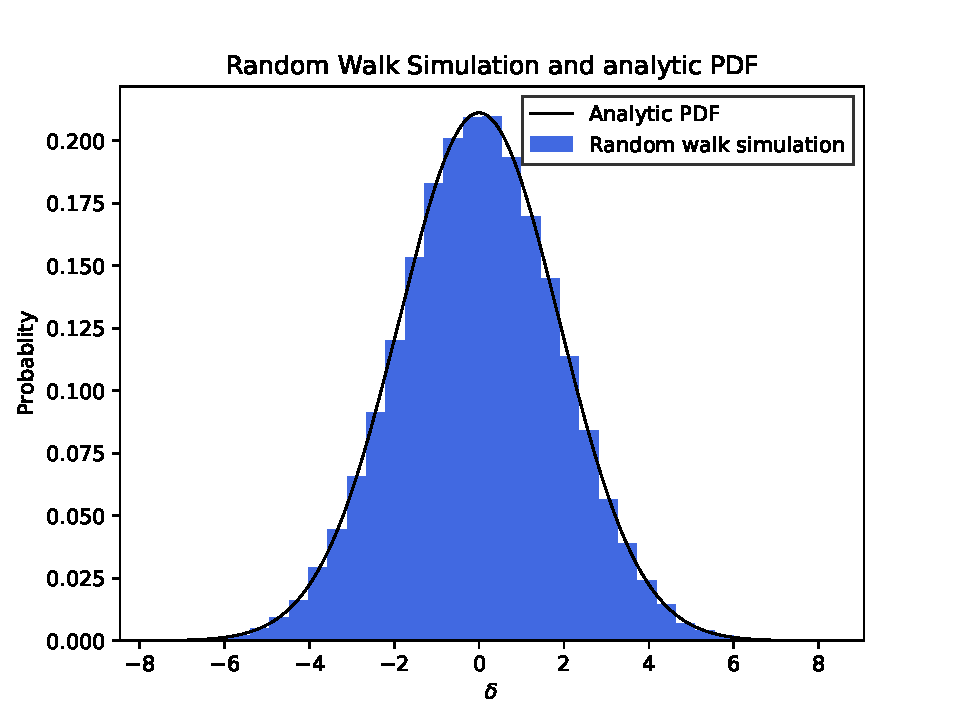
\includegraphics[width=0.8\linewidth]{Figures/randomwalk.pdf}
    \caption{Distribution of $10^5$  random walk realizations in addition to the Gaussian Probability distribution function (PDF).}
    \label{fig:2}
\end{figure}

\noindent We have also overplotted the analytic probability distribution for a Gaussian random field with overdensity $\delta$, smoothed by $S_c$ with a variance $\sigma^2$, which is given as

\begin{equation}\label{eq:8}
    P(\delta \mid M) = \frac{1}{\sqrt{2\pi}\sigma} \exp\left[ - \frac{\delta^2}{2\sigma^2} \right].
\end{equation}

\noindent We see that the analytic probability distribution perfectly represents the random walk simulation.

\newpage 

We can further choose to only study the chains which never crosses the threshold $\delta_\text{crit} = 1$. Analytically, the probability of this is given by

\begin{equation}\label{eq:9}
    P_\text{nc}(\delta \mid M) \frac{1}{\sqrt{2\pi}\sigma}\left( \exp\left[ - \frac{\delta^2}{2\sigma^2} \right] - \exp \left[ - \frac{[2\delta_\text{crit} - \delta]^2}{2\sigma^2} \right] \right).
\end{equation}

By editing our program to extract only $\delta <= 1$ We get the following distribution, with the analytic expression overplotted seen in figure \ref{fig:3}.

\begin{figure}[h]
    \centering
    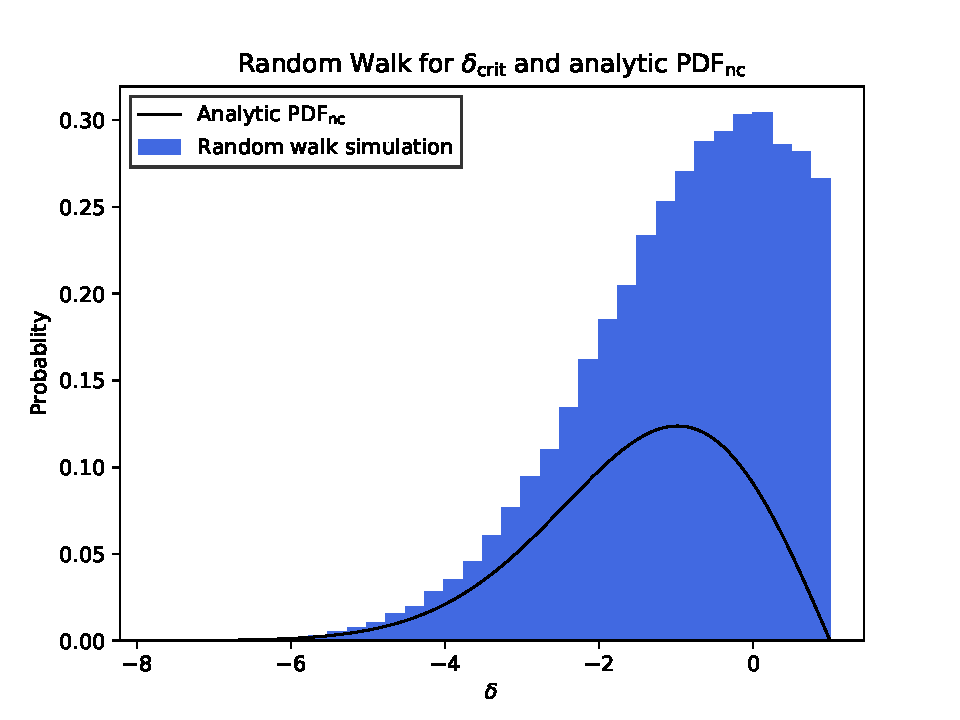
\includegraphics[width=0.8\linewidth]{Figures/randomcritwalk.pdf}
    \caption{Distribution of $10^5$ random walk realizations where only the chains up to $\delta \leq 1$ have been included. This is then compared to the analytic probability distribution PDF$_{nc}$.}
    \label{fig:3}
\end{figure}

\section*{Exercise 3.}
\subsection*{(1)}

From the analysis in exercise 2, we know that the probability distribution function for $\delta \leq \delta_\text{crit}$ at some scale $M' > M$ is given by equation \eqref{eq:9}. We know that the probability of finding mass larger than zero is given as

\[
    P(> 0) = P( > M) + P( < M) = 1.
\]

\noindent We can rewrite this to

\begin{equation}\label{eq:10}
    P( > M ) = 1 - P ( < M ).
\end{equation}

\noindent Mass smaller than $M$ corresponds to the density being smaller than critical overdensity $\delta_\text{crit}$. From the randomwalk analysis, we know that this has the probability of not crossing $P_\text{nc}$ seen in equation \eqref{eq:9}. By inserting this into the equation \eqref{eq:10} we get the following expression

\begin{equation}\label{eq:10}
    P(> M) = 1 - \int_{-\infty}^{\delta_\text{crit}} P_\text{nc} (\delta \mid M) d\delta,
\end{equation}

\noindent where we have integrated $P_\text{nc}$ from $-\infty$ to $\delta_\text{crit}$.

\subsection*{(2)}

We will now show how the factor 2 in the Press-Schechter formalism naturally occurs. We do so by first combingin equations \eqref{eq:9} and \eqref{eq:10}. This leaves us with 

\begin{equation}\label{eq:11}
    P(> M) = 1 - \frac{1}{\sqrt{2 \pi} \sigma} \int_{-\infty}^{\delta_\text{crit}} \left( \exp \left[- \frac{\delta^2}{2\sigma^2} \right] - \exp \left[ - \frac{[2\delta_\text{crit} - \delta]^2 }{2\sigma^2} \right] \right)
\end{equation}

\noindent We split the integral into two integrals, I and II

\[
     \text{I}:\qquad  \int_{-\infty}^{\delta_\text{crit}} e^{- \delta^2 /2 \sigma^2} d\delta,
\]

\[
    \text{II}:\qquad  \int_{-\infty}^{\delta_\text{crit}} e^{- (2\delta_\text{crit} - \delta)^2/2 \sigma^2} d\delta.
\]

\noindent We start with computing I

\[
    \text{I}:\qquad  \int_{-\infty}^{\delta_\text{crit}} e^{- \delta^2 /2 \sigma^2} d\delta = \frac{1}{2} \sqrt{2 \pi} \sigma\left[ \text{erf}  \left( \frac{\nu}{\sqrt{2}}\right) + 1 \right],
\]

\noindent where we have substituted $\nu = \delta_\text{crit}/ \sigma$, and erf is the error function given as 

\[
    \text{erf}(x) = \frac{2}{\sqrt{\pi}} \int_0^x e^{-t^2} dt.
\]

\noindent Similarely, we compute II

\[
    \text{II}:\qquad  \int_{-\infty}^{\delta_\text{crit}} e^{- (2\delta_\text{crit} - \delta)^2/2 \sigma^2} d\delta = \frac{1}{2} \sqrt{2 \pi} \sigma \; \text{erfc} \left( \frac{\nu}{\sqrt{2}}\right),
\]

\noindent where erfc is given as

\[
    \text{erfc}(x) = 1 - \text{erf}(x).
\]

\noindent We now solve the integral expression in equation \eqref{eq:11} by computing I - II

\begin{align*}
\text{I} - \text{II} \quad & = \quad   \frac{1}{2} \sqrt{2 \pi} \sigma\left[ \text{erf}  \left( \frac{\nu}{\sqrt{2}}\right) + 1 \right] - \frac{1}{2} \sqrt{2 \pi} \sigma \; \text{erfc} \left( \frac{\nu}{\sqrt{2}}\right)
\\
& = \quad \frac{1}{2} \sqrt{2\pi} \sigma \left[\text{erf}  \left( \frac{\nu}{\sqrt{2}}\right) + 1 - \text{erfc} \left( \frac{\nu}{\sqrt{2}}\right) \right]
\\
& = \quad \frac{1}{2} \sqrt{2\pi} \sigma \left[\text{erf}  \left( \frac{\nu}{\sqrt{2}}\right) + 1 - 1 + \text{erf} \left( \frac{\nu}{\sqrt{2}}\right) \right]
\\
& = \quad \sqrt{2\pi} \sigma \; \text{erf}  \left( \frac{\nu}{\sqrt{2}}\right)
\end{align*}

\noindent We can then insert this expression into the integral in equation \eqref{eq:11}, which leaves us with

\[
    P(> M) = 1 - \frac{1}{\sqrt{2 \pi} \sigma}\sqrt{2\pi} \sigma \; \text{erf}  \left( \frac{\nu}{\sqrt{2}}\right).
\]

\noindent We see that the factor $\sqrt{2\pi}\sigma$ disappears, and we are left with the Press-Schelter expression

\begin{equation}
     P(> M) = 1 - \text{erf}  \left( \frac{\nu}{\sqrt{2}}\right),
\end{equation}
where the factor $2$ now naturally comes in.


\end{document}